\documentclass[english]{article} 
\usepackage[absolute,overlay]{textpos} 
\usepackage{amsthm}
\usepackage{amsmath}
\usepackage{amssymb}
\usepackage[utf8]{inputenc}
\usepackage[english]{babel}
\usepackage{graphicx}
\usepackage{geometry}
\usepackage{caption}
\usepackage{subcaption}
\usepackage{pdfpages}
\usepackage{comment}
\usepackage{bm}
\usepackage{etoolbox}
\usepackage{mathtools}
\usepackage{tikz}

\usepackage{algpseudocode}
\usepackage{algorithm}
\usepackage{mathrsfs} 
\usepackage{multirow}

\usepackage{pgfplots}
\usepackage{pgfplotstable}
\usepackage{stmaryrd} 

\usepackage{hyperref}


\usepackage{booktabs}
\usepackage{makecell}

\usepackage{adjustbox}

\usepackage[noabbrev,capitalise]{cleveref}
\crefformat{appendix}{#2#1#3}

\usetikzlibrary{fillbetween}
\usepgfplotslibrary{fillbetween}

\usetikzlibrary{shapes.misc}
\usetikzlibrary{math} 

\usetikzlibrary{arrows}


\definecolor{darkspringgreen}{rgb}{0., 0.55, 0.3}
\definecolor{dartmouthgreen}{rgb}{0.05, 0.5, 0.06}
\definecolor{etonblue}{rgb}{0.59, 0.78, 0.64}
\definecolor{airforceblue}{rgb}{0., 0.4, 0.66}
\definecolor{arylideyellow}{rgb}{0.91, 0.84, 0.42}
\definecolor{emerald}{rgb}{0.31, 0.78, 0.47}
\definecolor{uclagold}{rgb}{1.0, 0.7, 0.0}
\definecolor{cadmiumorange}{rgb}{0.93, 0.53, 0.18}

\def\colorPalette{{"0.00 0.55 0.3","0.93 0.53 0.18","0.00 0.40 0.66","1.00 0.70 0.00","0.80 0.00 0.00","0.00 0.40 0.66", "0.05 0.50 0.06", "0.31 0.78 0.47", "0.59 0.78 0.64", "0.12 0.63 0.11", "0.75 0.43 0.1", "0.8 0.05 0.5"}}




%\newtheorem{theorem}{Theorem}
%\numberwithin{theorem}{section}
%\newtheorem{definition}{Definition}
%\numberwithin{definition}{section}
%\newtheorem{remark}{Remark}
%\numberwithin{remark}{section}
%\newtheorem{proposition}[theorem]{Proposition}
%\newtheorem{lemma}[theorem]{Lemma}
%\newtheorem{corollary}[theorem]{Corollary}

\theoremstyle{thmstyleone}
\newtheorem{theorem}{Theorem}
\newtheorem{proposition}[theorem]{Proposition}
\newtheorem{lemma}[theorem]{Lemma}
\newtheorem{corollary}[theorem]{Corollary}


\theoremstyle{thmstyletwo}
\newtheorem{example}{Example}
\newtheorem{remark}{Remark}

\theoremstyle{thmstylethree}
\newtheorem{definition}{Definition}


\newcommand{\lop}[0]{\mathcal{L}}
\newcommand{\lopd}[0]{\mathcal{L}_\Delta}
\newcommand{\lopdt}[0]{\mathcal{L}_{\Delta}}
\newcommand{\LL}{\lopdt}
\newcommand{\usol}[0]{\underline{\uvec{u}}_\Delta}
\newcommand{\usoldt}[0]{\underline{\uvec{u}}_\Delta}


\newcommand{\up}[0]{\underline{\uvec{u}}^{(p)}}

\newcommand{\usoldto}[0]{\tilde{\underline{\uvec{u}}}_\Delta}

\newcommand{\uapp}[0]{\uvec{u}_h}
\newcommand{\wapp}[0]{w_h}

\newcommand{\massmatrix}[0]{\mathcal{M}}

\newcommand{\tess}[0]{\mathcal{T}_h}


\newcommand{\uvec}[2][3]{\boldsymbol{#2\mkern-#1mu}\mkern#1mu}


\newcommand{\res}[0]{\textbf{R}}
\newcommand\norm[1]{\left\lVert#1\right\rVert}
\newcommand\abs[1]{\left\lvert#1\right\rvert}

\newcommand{\flux}[0]{\boldsymbol{F}}
\newcommand{\source}[0]{\boldsymbol{S}}
\newcommand{\ST}[0]{\boldsymbol{ST}_i^K}
\newcommand{\extra}[0]{\boldsymbol{ST}_i}


\newcommand{\elres}[0]{\uvec{\Phi}^K(\uapp)}
\newcommand{\noderes}[0]{\uvec{\Phi}^K_i(\uapp)}
%\newcommand{\spacestuff}[0]{\boldsymbol{\phi}_i}
\newcommand{\cund}[0]{\underline{\uvec{c}}}
\newcommand{\lopdi}[0]{\mathcal{L}_{\Delta,i}}
\newcommand{\csoldt}[0]{\underline{\uvec{c}}_\Delta}
\newcommand{\basis}[0]{\uvec{v}}
\newcommand{\mis}[0]{\mu}
\def\restriction#1#2{\mathchoice
              {\setbox1\hbox{${\displaystyle #1}_{\scriptstyle #2}$}
              \restrictionaux{#1}{#2}}
              {\setbox1\hbox{${\textstyle #1}_{\scriptstyle #2}$}
              \restrictionaux{#1}{#2}}
              {\setbox1\hbox{${\scriptstyle #1}_{\scriptscriptstyle #2}$}
              \restrictionaux{#1}{#2}}
              {\setbox1\hbox{${\scriptscriptstyle #1}_{\scriptscriptstyle #2}$}
              \restrictionaux{#1}{#2}}}
\def\restrictionaux#1#2{{#1\,\smash{\vrule height .8\ht1 depth .85\dp1}}_{\,#2}} 
\newcommand\swapifbranches[3]{#1{#3}{#2}}
\newcommand{\R}{\mathbb{R}}
\newcommand{\dt}{\Delta t}
\newcommand{\redun}[1]{{\color{red} {\large \textit{Is the following redundant?}} #1}}
\newcommand{\davide}[1]{{\color{purple}#1}}
\newcommand{\lore}[1]{ \textbf{{\color{blue}#1}}}
\newcommand{\question}[1]{{\color{red} \large Question: #1 }}
\newcommand{\bu}{\uvec{u}}
\newcommand{\bbu}{\underline{\uvec{u}}}
\newcommand{\bU}{\uvec{U}}
\newcommand{\bbU}{\underline{\uvec{U}}}
\newcommand{\bbr}{\underline{\uvec{r}}}
\newcommand{\by}{\uvec{y}}
\newcommand{\bby}{\underline{\uvec{y}}}
\newcommand{\bG}{{\uvec{G}}}
\newcommand{\bbt}{\underline{t}}
\newcommand{\vecz}{\underline{0}}
\newcommand{\matz}{\underline{\underline{0}}}
\newcommand{\vecbeta}{\underline{\beta}}
\newcommand{\CIP}{\text{CIP}}
\newcommand{\OSS}{\text{OSS}}
\newcommand{\CFL}{\text{CFL}}

\newcommand{\undu}{\underline{\uvec{u}}}
\newcommand{\undy}{\underline{\uvec{y}}}
\newcommand{\undspacetilde}{\widetilde{\underline{\uvec{\phi}}}}
\newcommand{\spacestuff}{\uvec{\phi}}
\newcommand{\undv}{\underline{\uvec{v}}}
\newcommand{\undw}{\underline{\uvec{w}}}
\newcommand{\undr}{\underline{\uvec{r}}}
\newcommand{\undz}{\underline{\uvec{z}}}
\newcommand{\lopdtp}[0]{\mathcal{L}_{\Delta,p}}
\newcommand{\usolp}[0]{\underline{\uvec{u}}_{\Delta}^{(p)}}
\newcommand{\Xp}[0]{X^{(p)}}
\newcommand{\Yp}[0]{Y^{(p)}}
\newcommand{\uex}[0]{\underline{\uvec{u}}_{ex}}
\newcommand{\uexp}[0]{\underline{\uvec{u}}_{ex}^{(p)}}
\newcommand{\lopdLp}[0]{\mathcal{L}_\Delta^{1,(p)}}
\newcommand{\lopdHp}[0]{\mathcal{L}_\Delta^{2,(p)}}
\newcommand{\embep}[0]{\mathcal{E}^{(p)}}
\newcommand{\projp}[0]{\Pi^{(p)}}
\newcommand{\trialspace}[1]{\varphi_{#1}} %phi space _i
\newcommand{\trialspaceiter}[2]{\varphi_{#1}^{#2}} %phi space _i
\newcommand{\trialtime}[1]{\psi^{#1}} %psi time ^m
\newcommand{\trialtimeiter}[2]{\psi^{#1,#2}} %psi time ^m
%THE FOLLOWING IS  ^l TO AVOID CONFUSION WITH u_n
\newcommand{\trialspacetime}[1]{\vartheta^{#1}} %theta space time 
\newcommand{\trialspacetimeiter}[2]{\vartheta^{#1,#2}}

%ADER-FV
\newcommand{\trialspaceFVp}[1]{\varphi_{#1}} %predictor
\newcommand{\trialspaceFVc}[1]{\lambda_{#1}} %corrector 
\newcommand{\APNPM}{{ADER-$\mathbb P_N \mathbb P_M$ }}

%Temperature
%\newcommand{\Temp}{\tau}
\newcommand{\Temp}{T}


\newcommand{\E}{\boldsymbol{E}}

\newcommand{\pnpm}[2]{\mathbb P_{#1}\mathbb P_{#2}}  %PNPM schemes

\newcommand{\RIcolor}[1]{{\leavevmode\color{black} #1}}
\newcommand{\RIIcolor}[1]{{\leavevmode\color{black} #1}}


%\DeclarePairedDelimiter\abs{\lvert}{\rvert}

\newcommand{\hpsi}{\widehat{\psi}}
\newcommand{\hphi}{\widehat{\varphi}}
\newcommand{\hl}{\widehat{\lambda}}
\newcommand{\hK}{\widehat{K}}
\newcommand{\hw}{\widehat{\omega}}

\newcommand{\xt}{\uvec{x},t}
\newcommand{\et}{\uvec{xi},t}

\begin{document}
\author{L. Micalizzi\footnote{Affiliation: Institute of Mathematics, University of Zurich, Winterthurerstrasse 190, Zurich, 8057, Switzerland. Email: lorenzo.micalizzi@math.uzh.ch.} }
\title{Spectral methods for Lagrangian Continuous FEM}  


\maketitle
%\tableofcontents

%\abstract{bla bla}

\section{Convention on the transformation}
Let us consider a space domain occupying a region $\Omega_0$ at time $t=0$. Its general point is denoted by $\uvec{X}\in \Omega_0$.
%
Then, we assume the existence of a map $\uvec{x}=\widetilde{\uvec{x}}(\uvec{X},t)$, associating to each $\uvec{X}$ a point $\uvec{x}\in \Omega_t$, where $\Omega_t$ is the image of $\Omega_0$ through $\widetilde{\uvec{x}}(\cdot,t)$.

Actually, for convenience, we will not work with the map $\widetilde{\uvec{x}}(\cdot,t):\Omega_0\rightarrow\Omega_t$, from the initial configuration $\Omega_0$ to $\Omega_t$, but rather with $\uvec{x}(\cdot,t):\widehat{\Omega}\rightarrow\Omega_t$, from a reference configuration $\widehat{\Omega}$ to $\Omega_t$.
The general point in $\widehat{\Omega}$ is denoted by $\uvec{\xi}$.
%
A sketch is reported in Figure \ref{fig:lagrangian_maps}. 
%
\begin{figure}
	\centering
	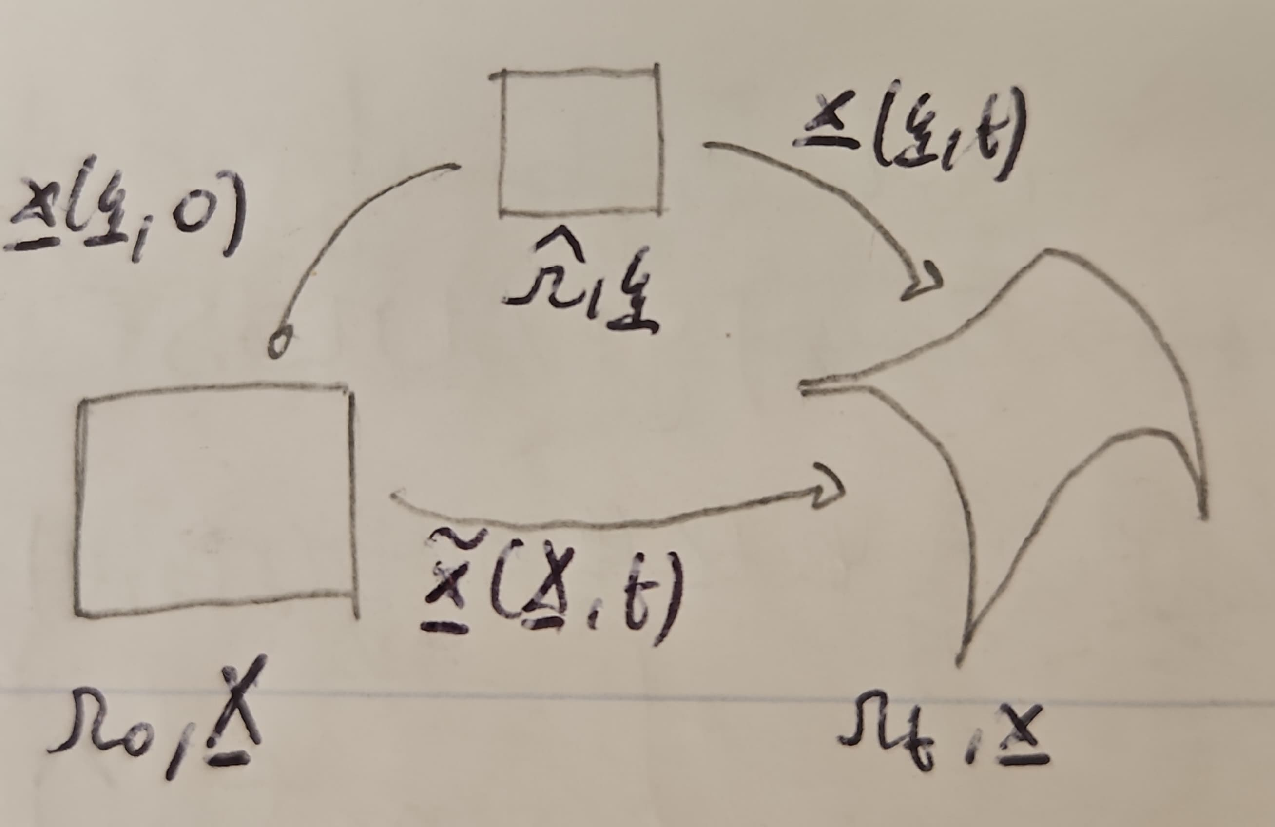
\includegraphics[width=0.4\textwidth]{lagrangian_maps.pdf}
	\caption{Sketch of the maps $\widetilde{\uvec{x}}(\uvec{X},t)$ and $\uvec{x}(\uvec{\xi},t)$}\label{fig:lagrangian_maps}
\end{figure}
%
Further, we define the deformation gradient $\uvec{J}(\uvec{\xi},t):=\nabla_{\uvec{\xi}}\uvec{x}(\uvec{\xi},t).$



\textcolor{red}{\textbf{Summarizing}, I work with a map $\uvec{x}(\uvec{\xi},t)$ from the reference configuration $\widehat{\Omega}$ to $\Omega_t$.}\\
\textcolor{blue}{\textbf{NB}: The notation is $2D$ because I understand it better this way, but I work in $1D$. So, for example, the deformation gradient is a scalar number $\uvec{J}(\uvec{\xi},t):=\nabla_{\uvec{\xi}}\uvec{x}(\uvec{\xi},t)=\frac{dx(\uvec{\xi},t)}{d\xi},$ coinciding hence with its determinant $det \uvec{J}(\uvec{\xi},t):=\frac{\partial x(\uvec{\xi},t)}{\partial \xi}.$}

\section{Governing equations}
The governing equations are
\begin{itemize}
\item \textbf{Deformation map}
\begin{equation}
\frac{d}{dt}\uvec{x}(\uvec{\xi},t)=\uvec{v}(\uvec{x}(\uvec{\xi},t),t);
\end{equation}

\item \textbf{Mass conservation}

\begin{align}
&H(\uvec{x}(\uvec{\xi},t),t)=\frac{\widehat{H}(\uvec{\xi})}{det \uvec{J}(\uvec{\xi},0)}\label{eq:strong_mass_conservation}%\\
%&\frac{d}{dt}H(\uvec{x},t)+H(\uvec{x},t)div_{\uvec{x}}\uvec{v}(\uvec{x},t)=0; \label{eq:weak_mass_conservation}
\end{align}

\item \textbf{Momentum conservation}
\begin{align}
&H\frac{d}{dt}\uvec{v}(\uvec{x},t)+gH\nabla_{\uvec{x}}\left(H(\uvec{x},t)+B(\uvec{x})\right)=\uvec{0}. \label{eq:momentum_wb}
\end{align}


\textcolor{red}{NB: I consider strong mass conservation (SMC)}\\
\textcolor{blue}{NB: In the velocity equation \textbf{I DO NOT simplify $H$}, otherwise conservation is lost and one does not converge to the weak solution. (At the beginning I coded the equation without $H$ and it was of course OK for smooth problems but not for shocks. I did not recover the correct shock location.)}



\end{itemize}


\section{Discretization}
The discretization of Dobrev, Tzanio and Rieben is assumed.
The thermodynamic variable $H_h$ is approximated in a discontinuous space of piecewise polynomial functions $\hpsi_i$ of degree $M$. Locally, we have
\begin{equation}
H_h(\uvec{\xi},t):=\sum_{i}H_i(t)\hpsi_i(\uvec{\xi}),
\end{equation}

The kinetic variables $\uvec{x}_h$ and $\uvec{v}_h$ are approximated in a continuous space of piecewise polynomial functions $\hphi_i$ of degree $M+1$. Globally, we have
\begin{align}
\uvec{x}_h(\uvec{\xi},t)&:=\sum_{i}\uvec{x}_i(t)\hphi_i(\uvec{\xi}),\\
\uvec{v}_h(\uvec{\xi},t)&:=\sum_{i}\uvec{v}_i(t)\hphi_i(\uvec{\xi}),
\end{align}


We define the basis functions on the trajectory of the motions $\psi_i(\uvec{x},t)$ and $\varphi_i(\uvec{x},t)$, in such a way that they are constant along the characteristics of the particles
\begin{align}
\varphi_i(\uvec{x},t)&:=\hphi_i(\uvec{\xi}(\uvec{x},t)),\\
\psi_i(\uvec{x},t)&:=\hpsi_i(\uvec{\xi}(\uvec{x},t)).
\end{align}

This allows to define the spatial description of the discretized variables
\begin{align*}
H_h(\uvec{x},t)&:=\sum_{i}H_i(t)\psi_i(\uvec{x},t)=\sum_{i}H_i(t)\hpsi_i(\uvec{\xi}(\uvec{x},t)),\\
\uvec{x}_h(\uvec{x},t)&:=\sum_{i}\uvec{x}_i(t)\varphi_i(\uvec{x},t)=\sum_{i}\uvec{x}_i(t)\hphi_i(\uvec{\xi}(\uvec{x},t)),\\
\uvec{v}_h(\uvec{x},t)&:=\sum_{i}\uvec{v}_i(t)\varphi_i(\uvec{x},t)=\sum_{i}\uvec{v}_i(t)\hphi_i(\uvec{\xi}(\uvec{x},t)),
\end{align*}
denoted, with abuse of notation, with the same symbols.

\textcolor{red}{\textbf{Summarizing},
\begin{align}
	H_h &\longrightarrow \left\lbrace \psi_i \right\rbrace~\text{discontinuous degree}~M \\
	\uvec{v}_h,\uvec{x}_h &\longrightarrow \left\lbrace \varphi_i \right\rbrace~\text{continuous degree}~M+1
\end{align}		
}

\section{Main point}\label{sec:main_point}
Q: Is it possible to achieve a proper mass lumping in Lagrangian, by adopting some spectral approach (special nodal bases with associated nodes used as quadrature points), e.g., Lagrange polynomials in the Gauss--Lobatto (GL) points?\\
A: Yes, BUT the (lumped) matrices will depend on time.

%We set $\lambda$ as a general handler for $\psi$ and $\varphi$ and we have
%\begin{align}
%\begin{split}
%\int_{K(t)} \lambda_i(\uvec{x},t)\lambda_j(\uvec{x},t)d\uvec{x}&=\int_{K(t)} \hl_i(\uvec{\xi},t)\hl_j(\uvec{\xi},t) det \uvec{J}(\uvec{\xi},t) d\uvec{\xi}\\
%&=\int_{\widehat{K}} \hl_i(\uvec{\xi},t)\hl_j(\uvec{\xi},t) det \uvec{J}(\uvec{\xi},t) d\uvec{\xi}\\
%&\approx \delta_{i,j}\widehat{\omega}_i det \uvec{J}(\uvec{\xi}_i,t)=M_{\lambda_i}^K(t).
%\end{split}
%\end{align}
%
%\textcolor{red}{
%NB: This is not the matrix that one integrates in Lagrangian, because one has usually to do with $\int_K H\lambda_i\lambda_j$.
%However, in SW, $H$ can be removed, see for example \eqref{eq:weak_mass_conservation} or \eqref{eq:momentum_wb}. Indeed, we can put it back by multiplying the equations by $H$.
%NEVERTHELESS, the lumping makes also the matrix $\int_K H\lambda_i\lambda_j$, which should be constant if one integrated it exactly, time-dependent.}

\begin{align}
\begin{split}
\int_{K(t)}H(\uvec{x},t) \lambda_i(\uvec{x},t)\lambda_j(\uvec{x},t)d\uvec{x}&=\int_{K(t)} \hl_i(\uvec{\xi},t)\hl_j(\uvec{\xi},t) det \uvec{J}(\uvec{\xi},t) d\uvec{\xi}\\
&=\int_{\widehat{K}}H(\uvec{\xi},t) \hl_i(\uvec{\xi},t)\hl_j(\uvec{\xi},t) det \uvec{J}(\uvec{\xi},t) d\uvec{\xi}\\
&\approx \delta_{i,j}H^K(\uvec{x}_i,t)\widehat{\omega}_i det \uvec{J}(\uvec{\xi}_i,t)=H^K(\uvec{x}_i,t)M_{\lambda_i}^K(t).
\end{split}
\end{align}

A time-dependent matrix may be a costly BUT, in the end, with the lumping it is just a point evaluation and becomes part of the ODE at the RHS!

\textcolor{red}{NB: $H^K(\uvec{x}_i,t)$ depends on the element as $H$ is discontinuous. (So, in the extrema of a segment $H^K(\uvec{x}_i,t)$ has 2 values)}


\section{Discrete equations}


\begin{itemize}
\item \textbf{Deformation map}

\begin{equation}
\frac{d}{dt}\uvec{x}_i(t)=\uvec{v}_i(t);
\end{equation}



\item \textbf{Mass conservation}

\begin{align}
&H_i(t)=\frac{\widehat{H}_i}{det \uvec{J}(\uvec{\xi}_i,0)}
\end{align}



\item \textbf{Momentum conservation}
\begin{align}
&H\frac{d}{dt}\uvec{v}(\uvec{x},t)+gH\nabla_{\uvec{x}}\left(H(\uvec{x},t)+B(\uvec{x})\right)=\uvec{0}, \label{eq:momentum_wb_bis}
\end{align}
\end{itemize}

discretized in a CG fashion as

\begin{equation}
\sum_{K \in K_i} H^K(\uvec{x}_i,t) M^K_{\varphi_i}(t)\frac{d}{dt}\uvec{v}_i(t)+g \sum_{K \in K_i} \int_K \varphi_i H_h\nabla_{\uvec{x}}(H_h+B_h)  d\uvec{x}=\uvec{0},
\end{equation}
leading to
\begin{equation}
\frac{d}{dt}\uvec{v}_i(t)=-\frac{1}{\sum_{K \in K_i} H^K(\uvec{x}_i,t) M^K_{\varphi_i}(t)}g \sum_{K \in K_i} \int_K \varphi_i H_h\nabla_{\uvec{x}}(H_h+B_h)  d\uvec{x}.
\end{equation}


\textcolor{red}{
NB: For me $K_i$ is the set of the elements containing the DoF $\uvec{x}_i$, which is well defined because we do not allow for connectivity changes.
}

Some coupling terms are needed in the velocity update for stability reasons (otherwise it is a central scheme)

\begin{equation}
	\frac{d}{dt}\uvec{v}_i(t)=-\frac{1}{\sum_{K \in K_i} H^K(\uvec{x}_i,t) M^K_{\varphi_i}(t)}\left(g \sum_{K \in K_i} \int_K \varphi_i H_h\nabla_{\uvec{x}}(H_h+B_h)  d\uvec{x} + \sum_{K \in K_i}\uvec{CT}^K_i(\uvec{u}_h) \right).
\end{equation}
We consider
\begin{align}
\begin{split}
\uvec{CT}^K_i(\uvec{u}_h):=\int_{\partial K} \varphi_i \overline{H_h} \left( \widehat{\eta}-\eta_h\vert_K \right) \uvec{\nu} d \uvec{\sigma}.
\end{split}
\label{eq:CT}
\end{align}
Actually, only the DoFs at the cell boundaries get such a contribution as they are the only ones not zero on $\partial K$. Moreover, the numerical flux $\widehat{\eta}$ simplifies when summing $\sum_{K \in K_i}$. In 1D one obtains, \textcolor{red}{\textbf{for DoFs at the cell boundaries only}}
\begin{align}
	\begin{split}
		\sum_{K \in K_i}\uvec{CT}^K_i(\uvec{u}_h) := \overline{H}_i \llbracket \eta \rrbracket_i,
	\end{split}
	\label{eq:CT1D}
\end{align}
while for the  internal DoFs of the cells one has no coupling contribution.


%CT_phi_v[global_indices_v[0]]=CT_phi_v[global_indices_v[0]]- ( (Hhat+Bhat)-(H_inside+B_inside) )*Hbar #IMPORTANT: - sign because of normal
%CT_phi_v[global_indices_v[-1]]=CT_phi_v[global_indices_v[-1]]+ ( (Hhat+Bhat)-(H_inside+B_inside) )*Hbar 


\section{Stabilization}

I have coded Burman on the velocity but it is not needed.
The coupling term seem to guarantee stability.
The convergence rates are obtained without Burman.
And Burman does not help with shocks.

%\begin{align}
%\uvec{ST}_i(\uapp)=\sum_f\sum_{r=1}^R \alpha_{f,r} \Bigg\llbracket \frac{\partial^r}{\partial x^r} \varphi_i \Bigg\rrbracket \cdot \Bigg\llbracket \frac{\partial^r}{\partial x^r} 
%\uvec{v}_h
% \Bigg\rrbracket 
%\label{eq:jt}
%\end{align}

\section{Boundary conditions}
When I assume periodic BCs there is no problem of course.

In the other cases, whenever something from outside the domain is needed, I use the state given by a Lagrangian Riemann solver (Eulerian Riemann solver along $\xi=v_{\text{boundary}}$).



\section{Time discretization}
I use DeC with GLB nodes with accuracy corresponding to the one of the space discretization.

\section{Tests}


\subsection{Accuracy}

I ran the same tests involving smooth moving equilibria of my Eulerian paper~\cite{micalizzi2023novel} with Mario and Rémi (with a $C^\infty$ compactly supported bathymetry).
The final time has been set to $T_f:=0.3$ in order to avoid the solution to flow out of the domain.
%
Results summarized in Tables~\ref{tab:supercritical}, \ref{tab:subcritical}, \ref{tab:transcritical}. I get the expected order.

Moreover, I ran an additional unsteady test without known solution. With periodic BCs on $[0,1]$, I consider the IC
\begin{align}
	\begin{split}
		\begin{cases}
			H(x,0)&:=2+\cos{(2 \pi x)},\\
			v(x,0)&:=1,
		\end{cases}
	\end{split}
\end{align}
and let the simulation evolve until the final time $T_f:=0.07$, short enough to avoid the formation of shocks.
%
The results are in in Table~\ref{tab:smooth_periodic}.
%
In this case, since the analytical solution is not know, I compute the error considering the values in the shared DoFs of sequences of meshes with half space size.
%
I get $2p$ for $x$ and $v$ for the "global flux argument" and expected order for $H$ and $q$.




	
%		\begin{tabular}{ | c| m{.1\textwidth} | c| m{.1\textwidth}  | c| m{.1\textwidth} | c| m{.1\textwidth}  | c| m{.1\textwidth} | c| m{.1\textwidth}  | c| m{.1\textwidth} | c| m{.1\textwidth}  | c| m{.1\textwidth} | c| m{.1\textwidth} |}


\begin{table}[ht]
	\centering
	\caption{Supercritical Smooth}
	\label{tab:supercritical}
	\begin{adjustbox}{width=1\textwidth}
	\small
		\begin{subtable}{1.\linewidth}
			\centering
			\caption{Order 2}
			\begin{tabular}{ccccccccccc}
				\toprule
				$N$ & $L^1(v)$ & Order $v$ & $L^1(H)$ & Order $H$ & $L^1(q)$ & Order $q$ & $\|v\|_2$ & Order $v$ & $\|H\|_2$ & Order $H$ \\
				\midrule
				10 & 1.744e-01 & 0.000 & 8.283e-02 & 0.000 & 8.101e-01 & 0.000 & 1.010e-02 & 0.000 & 4.802e-03 & 0.000 \\
				20 & 6.934e-02 & 1.331 & 3.134e-02 & 1.402 & 3.261e-01 & 1.313 & 4.430e-03 & 1.189 & 2.104e-03 & 1.191 \\
				40 & 2.349e-02 & 1.562 & 1.396e-02 & 1.167 & 1.104e-01 & 1.563 & 1.680e-03 & 1.399 & 9.405e-04 & 1.162 \\
				80 & 6.176e-03 & 1.927 & 3.713e-03 & 1.911 & 2.829e-02 & 1.964 & 4.485e-04 & 1.905 & 2.486e-04 & 1.920 \\
				160 & 1.215e-03 & 2.346 & 6.210e-04 & 2.580 & 5.172e-03 & 2.451 & 9.172e-05 & 2.290 & 4.128e-05 & 2.590 \\
				320 & 2.495e-04 & 2.284 & 7.725e-05 & 3.007 & 9.027e-04 & 2.518 & 1.986e-05 & 2.207 & 5.777e-06 & 2.837 \\
				\bottomrule
			\end{tabular}
		\end{subtable}
	\end{adjustbox}
	\begin{adjustbox}{width=1\textwidth}
	\small
		\begin{subtable}{1.\linewidth}
			\centering
			\caption{Order 3}
			\begin{tabular}{ccccccccccc}
				\toprule
				$N$ & $L^1(v)$ & Order $v$ & $L^1(H)$ & Order $H$ & $L^1(q)$ & Order $q$ & $\|v\|_2$ & Order $v$ & $\|H\|_2$ & Order $H$ \\
				\midrule
				10 & 7.715e-02 & 0.000 & 2.051e-02 & 0.000 & 2.496e-01 & 0.000 & 5.540e-03 & 0.000 & 1.965e-03 & 0.000 \\
				20 & 2.817e-02 & 1.454 & 1.154e-02 & 0.830 & 9.477e-02 & 1.397 & 2.174e-03 & 1.350 & 1.125e-03 & 0.805 \\
				40 & 6.022e-03 & 2.226 & 4.248e-03 & 1.442 & 3.041e-02 & 1.640 & 5.748e-04 & 1.919 & 4.764e-04 & 1.240 \\
				80 & 1.216e-03 & 2.308 & 8.815e-04 & 2.269 & 7.873e-03 & 1.950 & 8.951e-05 & 2.683 & 9.535e-05 & 2.321 \\
				160 & 1.683e-04 & 2.853 & 9.403e-05 & 3.229 & 1.125e-03 & 2.807 & 1.329e-05 & 2.752 & 8.819e-06 & 3.435 \\
				320 & 1.019e-05 & 4.046 & 6.467e-06 & 3.862 & 7.337e-05 & 3.939 & 8.702e-07 & 3.933 & 6.961e-07 & 3.663 \\
				\bottomrule
			\end{tabular}
		\end{subtable}
	\end{adjustbox}
	\begin{adjustbox}{width=1\textwidth}
	\small
		\begin{subtable}{1.\linewidth}
			\centering
			\caption{Order 4}
			\begin{tabular}{cccccccccccc}
				\toprule
				$N$ & $L^1(v)$ & Order $v$ & $L^1(H)$ & Order $H$ & $L^1(q)$ & Order $q$ & $\|v\|_2$ & Order $v$ & $\|H\|_2$ & Order $H$ \\
				\midrule
				10 & 2.878e-02 & 0.000 & 1.825e-02 & 0.000 & 1.490e-01 & 0.000 & 3.461e-03 & 0.000 & 3.129e-03 & 0.000 \\
				20 & 1.238e-02 & 1.217 & 5.741e-03 & 1.669 & 4.217e-02 & 1.821 & 1.710e-03 & 1.017 & 1.153e-03 & 1.440 \\
				40 & 2.113e-03 & 2.551 & 1.119e-03 & 2.359 & 8.343e-03 & 2.338 & 3.537e-04 & 2.273 & 2.308e-04 & 2.321 \\
				80 & 2.623e-04 & 3.010 & 1.310e-04 & 3.095 & 9.956e-04 & 3.067 & 3.436e-05 & 3.364 & 2.264e-05 & 3.350 \\
				160 & 1.756e-05 & 3.901 & 8.359e-06 & 3.970 & 1.077e-04 & 3.209 & 1.518e-06 & 4.500 & 1.009e-06 & 4.488 \\
				320 & 8.047e-07 & 4.448 & 4.131e-07 & 4.339 & 5.977e-06 & 4.171 & 5.709e-08 & 4.733 & 3.544e-08 & 4.831 \\
				\bottomrule
			\end{tabular}
		\end{subtable}
	\end{adjustbox}
	\begin{adjustbox}{width=1\textwidth}
	\small
		\begin{subtable}{1.\linewidth}
			\centering
			\caption{Order 5}
			\begin{tabular}{cccccccccccc}
				\toprule
				$N$ & $L^1(v)$ & Order $v$ & $L^1(H)$ & Order $H$ & $L^1(q)$ & Order $q$ & $\|v\|_2$ & Order $v$ & $\|H\|_2$ & Order $H$ \\
				\midrule
				10 & 2.446e-02 & 0.000 & 8.035e-03 & 0.000 & 9.873e-02 & 0.000 & 4.024e-03 & 0.000 & 1.814e-03 & 0.000 \\
				20 & 5.208e-03 & 2.232 & 2.753e-03 & 1.545 & 2.421e-02 & 2.028 & 8.839e-04 & 2.187 & 6.388e-04 & 1.506 \\
				40 & 8.040e-04 & 2.695 & 3.425e-04 & 3.007 & 3.515e-03 & 2.784 & 1.373e-04 & 2.687 & 8.175e-05 & 2.966 \\
				80 & 7.411e-05 & 3.439 & 3.108e-05 & 3.462 & 2.703e-04 & 3.701 & 8.558e-06 & 4.004 & 6.181e-06 & 3.725 \\
				160 & 3.023e-06 & 4.616 & 1.432e-06 & 4.440 & 1.180e-05 & 4.518 & 2.822e-07 & 4.922 & 2.366e-07 & 4.707 \\
				320 & 4.968e-08 & 5.927 & 2.336e-08 & 5.938 & 2.736e-07 & 5.431 & 4.049e-09 & 6.123 & 3.266e-09 & 6.179 \\
				\bottomrule
			\end{tabular}
		\end{subtable}
	\end{adjustbox}
\end{table}


\begin{table}[ht]
	\centering
	\caption{Subcritical Smooth}
	\label{tab:subcritical}
	\begin{adjustbox}{width=1\textwidth}
		\small
		\begin{subtable}{1.\linewidth}
			\centering
			\caption{Order 2}
			\begin{tabular}{ccccccccccc}
				\toprule
				$N$ & $L^1(v)$ & Order $v$ & $L^1(H)$ & Order $H$ & $L^1(q)$ & Order $q$ & $\|v\|_2$ & Order $v$ & $\|H\|_2$ & Order $H$ \\
				\midrule
				10 & 2.109e-01 & 0.000 & 1.240e-01 & 0.000 & 5.223e-01 & 0.000 & 1.823e-02 & 0.000 & 8.543e-03 & 0.000 \\
				20 & 7.270e-02 & 1.537 & 3.023e-02 & 2.036 & 2.040e-01 & 1.356 & 6.775e-03 & 1.428 & 2.494e-03 & 1.776 \\
				40 & 1.804e-02 & 2.011 & 9.276e-03 & 1.704 & 4.210e-02 & 2.277 & 1.678e-03 & 2.013 & 7.661e-04 & 1.703 \\
				80 & 4.888e-03 & 1.884 & 1.616e-03 & 2.521 & 1.114e-02 & 1.918 & 4.548e-04 & 1.883 & 1.469e-04 & 2.383 \\
				160 & 1.231e-03 & 1.989 & 3.632e-04 & 2.154 & 2.694e-03 & 2.048 & 1.142e-04 & 1.994 & 3.426e-05 & 2.100 \\
				320 & 3.101e-04 & 1.989 & 9.025e-05 & 2.009 & 6.739e-04 & 1.999 & 2.895e-05 & 1.980 & 8.500e-06 & 2.011 \\
				\bottomrule
			\end{tabular}
		\end{subtable}
	\end{adjustbox}
	\begin{adjustbox}{width=1\textwidth}
		\small
		\begin{subtable}{1.\linewidth}
			\centering
			\caption{Order 3}
				\begin{tabular}{ccccccccccc}
					\toprule
					$N$ & $L^1(v)$ & Order $v$ & $L^1(H)$ & Order $H$ & $L^1(q)$ & Order $q$ & $\|v\|_2$ & Order $v$ & $\|H\|_2$ & Order $H$ \\
					\midrule
					10 & 6.550e-02 & 0.000 & 3.025e-02 & 0.000 & 1.948e-01 & 0.000 & 5.156e-03 & 0.000 & 3.223e-03 & 0.000 \\
					20 & 1.550e-02 & 2.079 & 7.137e-03 & 2.084 & 4.629e-02 & 2.073 & 1.283e-03 & 2.007 & 8.902e-04 & 1.856 \\
					40 & 1.981e-03 & 2.968 & 1.119e-03 & 2.673 & 8.155e-03 & 2.505 & 1.865e-04 & 2.782 & 9.616e-05 & 3.211 \\
					80 & 3.017e-04 & 2.715 & 1.349e-04 & 3.052 & 8.817e-04 & 3.209 & 2.675e-05 & 2.802 & 1.261e-05 & 2.931 \\
					160 & 1.719e-05 & 4.133 & 8.177e-06 & 4.044 & 7.247e-05 & 3.605 & 1.733e-06 & 3.948 & 1.161e-06 & 3.441 \\
					320 & 1.068e-06 & 4.009 & 6.866e-07 & 3.574 & 7.262e-06 & 3.319 & 1.468e-07 & 3.561 & 1.362e-07 & 3.092 \\
					\bottomrule
				\end{tabular}
		\end{subtable}
	\end{adjustbox}
	\begin{adjustbox}{width=1\textwidth}
		\small
		\begin{subtable}{1.\linewidth}
			\centering
			\caption{Order 4}
			\begin{tabular}{ccccccccccc}
				\toprule
				$N$ & $L^1(v)$ & Order $v$ & $L^1(H)$ & Order $H$ & $L^1(q)$ & Order $q$ & $\|v\|_2$ & Order $v$ & $\|H\|_2$ & Order $H$ \\
				\midrule
				10 & 3.076e-02 & 0.000 & 1.696e-02 & 0.000 & 9.183e-02 & 0.000 & 3.086e-03 & 0.000 & 1.635e-03 & 0.000 \\
				20 & 4.355e-03 & 2.820 & 2.626e-03 & 2.691 & 1.553e-02 & 2.564 & 4.041e-04 & 2.933 & 2.306e-04 & 2.826 \\
				40 & 6.593e-04 & 2.724 & 2.809e-04 & 3.225 & 1.807e-03 & 3.103 & 6.003e-05 & 2.751 & 2.975e-05 & 2.954 \\
				80 & 3.369e-05 & 4.291 & 1.430e-05 & 4.296 & 1.192e-04 & 3.922 & 3.545e-06 & 4.082 & 1.944e-06 & 3.936 \\
				160 & 1.245e-06 & 4.758 & 5.833e-07 & 4.616 & 4.815e-06 & 4.630 & 1.245e-07 & 4.832 & 8.744e-08 & 4.475 \\
				320 & 4.355e-08 & 4.837 & 2.672e-08 & 4.448 & 2.301e-07 & 4.387 & 4.595e-09 & 4.760 & 4.952e-09 & 4.142 \\
				\bottomrule
			\end{tabular}
		\end{subtable}
	\end{adjustbox}
	\begin{adjustbox}{width=1\textwidth}
		\small
		\begin{subtable}{1.\linewidth}
			\centering
			\caption{Order 5}
			\begin{tabular}{ccccccccccc}
				\toprule
				$N$ & $L^1(v)$ & Order $v$ & $L^1(H)$ & Order $H$ & $L^1(q)$ & Order $q$ & $\|v\|_2$ & Order $v$ & $\|H\|_2$ & Order $H$ \\
				\midrule
				10 & 1.466e-02 & 0.000 & 7.934e-03 & 0.000 & 4.282e-02 & 0.000 & 1.173e-03 & 0.000 & 6.095e-04 & 0.000 \\
				20 & 2.056e-03 & 2.834 & 1.078e-03 & 2.880 & 6.227e-03 & 2.782 & 2.173e-04 & 2.432 & 1.071e-04 & 2.509 \\
				40 & 1.683e-04 & 3.611 & 7.934e-05 & 3.764 & 5.948e-04 & 3.388 & 1.670e-05 & 3.702 & 7.890e-06 & 3.763 \\
				80 & 5.894e-06 & 4.836 & 2.476e-06 & 5.002 & 1.936e-05 & 4.941 & 6.140e-07 & 4.765 & 3.019e-07 & 4.708 \\
				160 & 9.745e-08 & 5.918 & 4.522e-08 & 5.775 & 3.962e-07 & 5.611 & 1.007e-08 & 5.930 & 7.287e-09 & 5.373 \\
				320 & 2.202e-09 & 5.468 & 1.166e-09 & 5.277 & 1.039e-08 & 5.253 & 2.993e-10 & 5.072 & 2.921e-10 & 4.641 \\
				\bottomrule
			\end{tabular}
		\end{subtable}
	\end{adjustbox}
\end{table}




\begin{table}[ht]
	\centering
	\caption{Transcritical Smooth}
	\label{tab:transcritical}
	\begin{adjustbox}{width=1\textwidth}
		\small
		\begin{subtable}{1.\linewidth}
			\centering
			\caption{Order 2}
			\begin{tabular}{ccccccccccc}
				\toprule
				$N$ & $L^1(v)$ & Order $v$ & $L^1(H)$ & Order $H$ & $L^1(q)$ & Order $q$ & $\|v\|_2$ & Order $v$ & $\|H\|_2$ & Order $H$ \\
				\midrule
				10 & 3.335e-01 & 0.000 & 8.740e-02 & 0.000 & 3.794e-01 & 0.000 & 3.122e-02 & 0.000 & 5.406e-03 & 0.000 \\
				20 & 1.144e-01 & 1.544 & 2.943e-02 & 1.570 & 1.132e-01 & 1.745 & 9.630e-03 & 1.697 & 2.305e-03 & 1.230 \\
				40 & 3.917e-02 & 1.546 & 6.305e-03 & 2.223 & 2.890e-02 & 1.970 & 3.751e-03 & 1.360 & 5.204e-04 & 2.147 \\
				80 & 1.001e-02 & 1.968 & 1.771e-03 & 1.832 & 7.595e-03 & 1.928 & 9.108e-04 & 2.042 & 1.727e-04 & 1.591 \\
				160 & 2.435e-03 & 2.039 & 3.754e-04 & 2.238 & 1.778e-03 & 2.095 & 2.279e-04 & 1.999 & 3.656e-05 & 2.240 \\
				320 & 6.098e-04 & 1.998 & 8.831e-05 & 2.088 & 4.478e-04 & 1.989 & 5.710e-05 & 1.997 & 8.306e-06 & 2.138 \\
				\bottomrule
			\end{tabular}
		\end{subtable}
	\end{adjustbox}
	\begin{adjustbox}{width=1\textwidth}
		\small
		\begin{subtable}{1.\linewidth}
			\centering
			\caption{Order 3}
			\begin{tabular}{ccccccccccc}
				\toprule
				$N$ & $L^1(v)$ & Order $v$ & $L^1(H)$ & Order $H$ & $L^1(q)$ & Order $q$ & $\|v\|_2$ & Order $v$ & $\|H\|_2$ & Order $H$ \\
				\midrule
				10 & 9.984e-02 & 0.000 & 2.604e-02 & 0.000 & 8.318e-02 & 0.000 & 8.870e-03 & 0.000 & 3.695e-03 & 0.000 \\
				20 & 3.271e-02 & 1.610 & 7.147e-03 & 1.865 & 2.613e-02 & 1.671 & 2.882e-03 & 1.622 & 7.098e-04 & 2.380 \\
				40 & 3.919e-03 & 3.061 & 1.552e-03 & 2.203 & 4.952e-03 & 2.400 & 4.201e-04 & 2.778 & 2.415e-04 & 1.555 \\
				80 & 8.492e-04 & 2.206 & 2.150e-04 & 2.852 & 9.690e-04 & 2.353 & 1.177e-04 & 1.836 & 3.273e-05 & 2.883 \\
				160 & 7.962e-05 & 3.415 & 2.560e-05 & 3.070 & 1.022e-04 & 3.245 & 1.236e-05 & 3.251 & 4.617e-06 & 2.826 \\
				320 & 5.310e-06 & 3.906 & 2.236e-06 & 3.517 & 8.589e-06 & 3.573 & 1.007e-06 & 3.618 & 5.453e-07 & 3.082 \\
				\bottomrule
			\end{tabular}
		\end{subtable}
	\end{adjustbox}
	\begin{adjustbox}{width=1\textwidth}
		\small
		\begin{subtable}{1.\linewidth}
			\centering
			\caption{Order 4}
			\begin{tabular}{ccccccccccc}
				\toprule
				$N$ & $L^1(v)$ & Order $v$ & $L^1(H)$ & Order $H$ & $L^1(q)$ & Order $q$ & $\|v\|_2$ & Order $v$ & $\|H\|_2$ & Order $H$ \\
				\midrule
				10 & 5.648e-02 & 0.000 & 1.225e-02 & 0.000 & 4.446e-02 & 0.000 & 6.378e-03 & 0.000 & 1.422e-03 & 0.000 \\
				20 & 7.042e-03 & 3.004 & 2.150e-03 & 2.510 & 6.359e-03 & 2.806 & 7.853e-04 & 3.022 & 6.761e-04 & 1.073 \\
				40 & 1.401e-03 & 2.330 & 2.804e-04 & 2.939 & 1.102e-03 & 2.529 & 2.906e-04 & 1.434 & 5.674e-05 & 3.575 \\
				80 & 8.771e-05 & 3.998 & 2.497e-05 & 3.489 & 9.448e-05 & 3.544 & 1.645e-05 & 4.143 & 6.958e-06 & 3.028 \\
				160 & 6.607e-06 & 3.731 & 1.930e-06 & 3.694 & 8.749e-06 & 3.433 & 9.914e-07 & 4.052 & 4.411e-07 & 3.979 \\
				320 & 3.074e-07 & 4.426 & 9.881e-08 & 4.288 & 4.172e-07 & 4.390 & 4.589e-08 & 4.433 & 2.216e-08 & 4.315 \\
				\bottomrule
			\end{tabular}
		\end{subtable}
	\end{adjustbox}
	\begin{adjustbox}{width=1\textwidth}
		\small
		\begin{subtable}{1.\linewidth}
			\centering
			\caption{Order 5}
			\begin{tabular}{ccccccccccc}
				\toprule
				$N$ & $L^1(v)$ & Order $v$ & $L^1(H)$ & Order $H$ & $L^1(q)$ & Order $q$ & $\|v\|_2$ & Order $v$ & $\|H\|_2$ & Order $H$ \\
				\midrule
				10 & 2.143e-02 & 0.000 & 5.760e-03 & 0.000 & 1.930e-02 & 0.000 & 2.669e-03 & 0.000 & 1.215e-03 & 0.000 \\
				20 & 2.624e-03 & 3.030 & 9.996e-04 & 2.527 & 3.299e-03 & 2.549 & 5.025e-04 & 2.409 & 3.462e-04 & 1.811 \\
				40 & 4.733e-04 & 2.471 & 9.065e-05 & 3.463 & 3.197e-04 & 3.367 & 9.318e-05 & 2.431 & 3.428e-05 & 3.336 \\
				80 & 2.193e-05 & 4.432 & 9.440e-06 & 3.263 & 2.636e-05 & 3.600 & 3.754e-06 & 4.634 & 2.697e-06 & 3.668 \\
				160 & 8.913e-07 & 4.621 & 1.771e-07 & 5.736 & 6.981e-07 & 5.239 & 1.477e-07 & 4.668 & 4.562e-08 & 5.886 \\
				320 & 1.809e-08 & 5.623 & 5.593e-09 & 4.985 & 2.259e-08 & 4.950 & 2.811e-09 & 5.715 & 1.441e-09 & 4.985 \\
				\bottomrule
			\end{tabular}
		\end{subtable}
	\end{adjustbox}
\end{table}


\begin{table}[ht]
	\centering
	\caption{Smooth periodic}
	\label{tab:smooth_periodic}
	\begin{adjustbox}{width=1\textwidth}
		\small
		\begin{subtable}{1.\linewidth}
			\centering
			\caption{Order 2}
			\begin{tabular}{ccccccccccc}
				\toprule
				$N$ & Error $x$ & Order $x$ & Error $v$ & Order $v$ & Error $H$ & Order $H$ & Error $q$ & Order $q$ & Error $\eta$ & Order $\eta$ \\
				\midrule
				20 & 1.784e-03 & 0.000 & 4.913e-02 & 0.000 & 1.707e-02 & 0.000 & 1.235e-01 & 0.000 & 1.707e-02 & 0.000 \\
				40 & 4.451e-04 & 2.003 & 1.570e-02 & 1.646 & 5.601e-03 & 1.608 & 3.983e-02 & 1.632 & 5.601e-03 & 1.608 \\
				80 & 1.114e-04 & 1.998 & 4.700e-03 & 1.740 & 1.036e-03 & 2.435 & 1.152e-02 & 1.790 & 1.036e-03 & 2.435 \\
				160 & 2.799e-05 & 1.994 & 1.186e-03 & 1.987 & 2.625e-04 & 1.980 & 2.940e-03 & 1.970 & 2.625e-04 & 1.980 \\
				320 & 7.015e-06 & 1.996 & 2.963e-04 & 2.000 & 6.927e-05 & 1.922 & 7.413e-04 & 1.988 & 6.927e-05 & 1.922 \\
				\bottomrule
			\end{tabular}
		\end{subtable}
	\end{adjustbox}
	\begin{adjustbox}{width=1\textwidth}
		\small
		\begin{subtable}{1.\linewidth}
			\centering
			\caption{Order 3}
			\begin{tabular}{ccccccccccc}
				\toprule
				$N$ & Error $x$ & Order $x$ & Error $v$ & Order $v$ & Error $H$ & Order $H$ & Error $q$ & Order $q$ & Error $\eta$ & Order $\eta$ \\
				\midrule
				20 & 7.343e-05 & 0.000 & 4.707e-03 & 0.000 & 4.147e-03 & 0.000 & 1.393e-02 & 0.000 & 4.147e-03 & 0.000 \\
				40 & 6.320e-06 & 3.538 & 1.173e-03 & 2.005 & 8.122e-04 & 2.352 & 3.249e-03 & 2.100 & 8.122e-04 & 2.352 \\
				80 & 3.779e-07 & 4.064 & 8.200e-05 & 3.839 & 7.710e-05 & 3.397 & 2.141e-04 & 3.924 & 7.710e-05 & 3.397 \\
				160 & 2.287e-08 & 4.047 & 9.921e-06 & 3.047 & 1.367e-05 & 2.496 & 4.052e-05 & 2.401 & 1.367e-05 & 2.496 \\
				320 & 1.473e-09 & 3.956 & 7.446e-07 & 3.736 & 9.894e-07 & 3.788 & 3.008e-06 & 3.752 & 9.894e-07 & 3.788 \\
				\bottomrule
			\end{tabular}
		\end{subtable}
	\end{adjustbox}
	\begin{adjustbox}{width=1\textwidth}
		\small
		\begin{subtable}{1.\linewidth}
			\centering
			\caption{Order 4}
			\begin{tabular}{ccccccccccc}
				\toprule
				$N$ & Error $x$ & Order $x$ & Error $v$ & Order $v$ & Error $H$ & Order $H$ & Error $q$ & Order $q$ & Error $\eta$ & Order $\eta$ \\
				\midrule
				20 & 1.529e-05 & 0.000 & 2.305e-03 & 0.000 & 4.598e-04 & 0.000 & 6.164e-03 & 0.000 & 4.598e-04 & 0.000 \\
				40 & 8.267e-07 & 4.209 & 1.916e-04 & 3.589 & 1.083e-04 & 2.086 & 3.774e-04 & 4.030 & 1.083e-04 & 2.086 \\
				80 & 2.491e-08 & 5.052 & 1.621e-05 & 3.563 & 3.160e-05 & 1.777 & 6.600e-05 & 2.515 & 3.160e-05 & 1.777 \\
				160 & 3.503e-10 & 6.152 & 2.755e-07 & 5.879 & 3.805e-06 & 3.054 & 6.827e-06 & 3.273 & 3.805e-06 & 3.054 \\
				320 & 4.078e-12 & 6.425 & 4.103e-09 & 6.069 & 2.796e-07 & 3.767 & 5.111e-07 & 3.740 & 2.796e-07 & 3.767 \\
				\bottomrule
			\end{tabular}
		\end{subtable}
	\end{adjustbox}
	\begin{adjustbox}{width=1\textwidth}
		\small
		\begin{subtable}{1.\linewidth}
			\centering
			\caption{Order 5}
			\begin{tabular}{ccccccccccc}
				\toprule
				$N$ & Error $x$ & Order $x$ & Error $v$ & Order $v$ & Error $H$ & Order $H$ & Error $q$ & Order $q$ & Error $\eta$ & Order $\eta$ \\
				\midrule
				20 & 3.881e-06 & 0.000 & 1.289e-03 & 0.000 & 8.883e-04 & 0.000 & 3.621e-03 & 0.000 & 8.883e-04 & 0.000 \\
				40 & 1.373e-07 & 4.821 & 6.116e-05 & 4.398 & 1.026e-04 & 3.114 & 1.719e-04 & 4.397 & 1.026e-04 & 3.114 \\
				80 & 1.334e-09 & 6.686 & 1.372e-06 & 5.478 & 4.221e-06 & 4.604 & 7.751e-06 & 4.471 & 4.221e-06 & 4.604 \\
				160 & 4.968e-12 & 8.068 & 6.953e-09 & 7.624 & 2.097e-07 & 4.331 & 3.898e-07 & 4.313 & 2.097e-07 & 4.331 \\
				320 & 2.670e-14 & 7.540 & 8.801e-11 & 6.304 & 5.524e-09 & 5.247 & 1.015e-08 & 5.263 & 5.524e-09 & 5.247 \\
				\bottomrule
			\end{tabular}
		\end{subtable}
	\end{adjustbox}
\end{table}



\subsection{WB}
Note that the scheme is naturally WB towards lake at rest.
I get machine precision for lake at rest (results omitted).

Furthermore, I considered the classical perturbation analysis on the non-smooth parabolic $C^0$ bathymetry
\begin{equation}
	B(x):=\begin{cases}
		0.2-0.05(x-10)^2, &\text{if}~8<x<12,\\
		0, & \text{otherwise}.
	\end{cases}
	\label{eq:c0_bathymetry}
\end{equation}

I have introduced the perturbation
\begin{equation}
	\eta(x):=\begin{cases}
		\eta_{s}+A\exp{\left(1-\frac{1}{1-\left(\frac{x-6}{0.5}\right)^2}\right)}, &\text{if}~5.5<x<6.5,\\
		\eta_{s}, & \text{otherwise},
	\end{cases}
	\label{eq:perturbation_lake_at_rest}
\end{equation}
with $A:=5\cdot 10^{-5}$, where $\eta_{s}\equiv 0.5$

Results reported in Figure~\ref{fig:LatR_perturbation}. They are OK.

\begin{figure}
	\centering
	\begin{subfigure}{0.40\textwidth}
		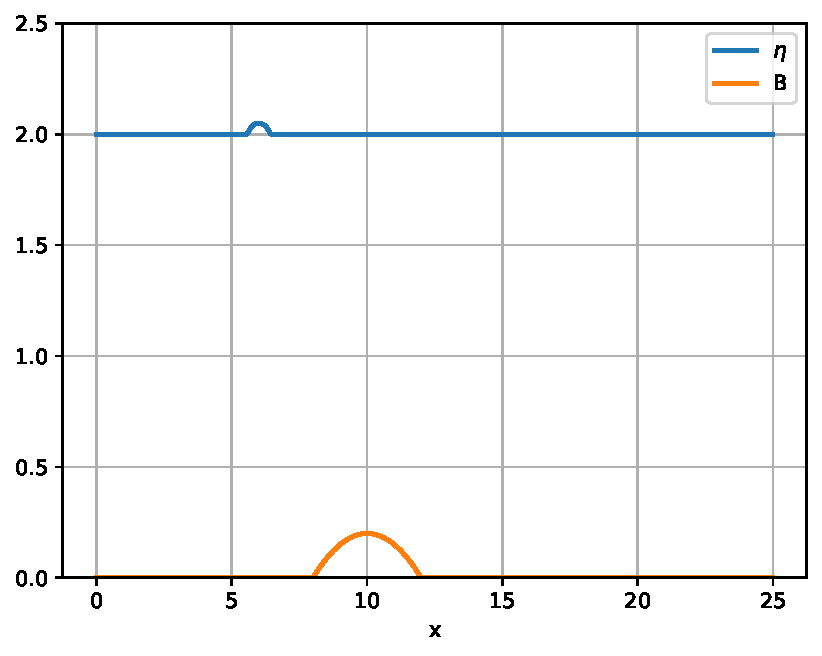
\includegraphics[width=\textwidth]{figures/25_LAKEATRESTNONSMOOTH.pdf}\caption{Initial total height and bathymetry. The perturbation is amplified by a factor $10^3$ in order to make it visible}
	\end{subfigure}
	\begin{subfigure}{0.40\textwidth}
		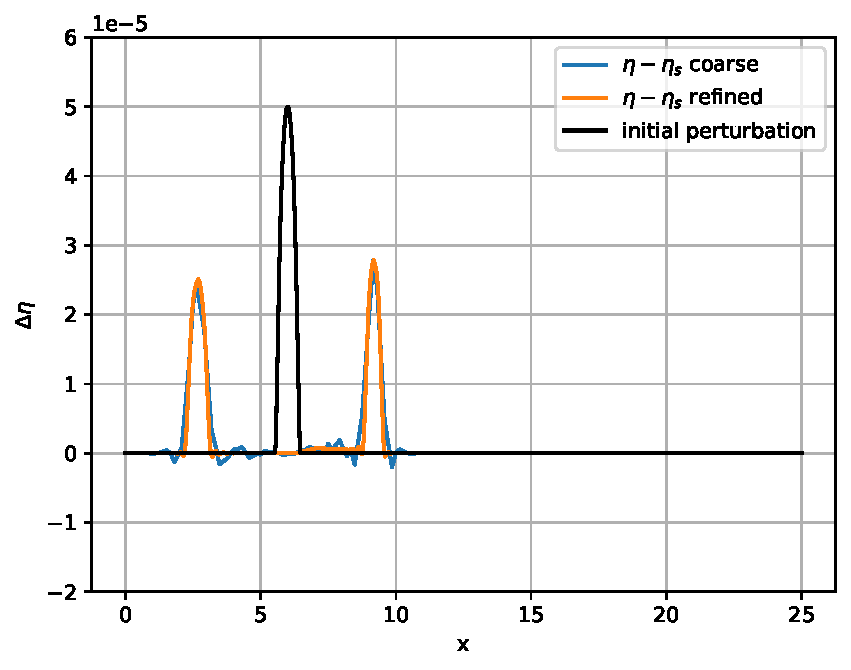
\includegraphics[width=\textwidth]{figures/31_LatRNSWBp3s14jt.pdf}\caption{Reference results with WB-HS and jr in the Eulerian paper with PGL and $30$ elements for the coarse mesh and $128$ for the refined one}
	\end{subfigure}\\
	\begin{subfigure}{0.60\textwidth}
		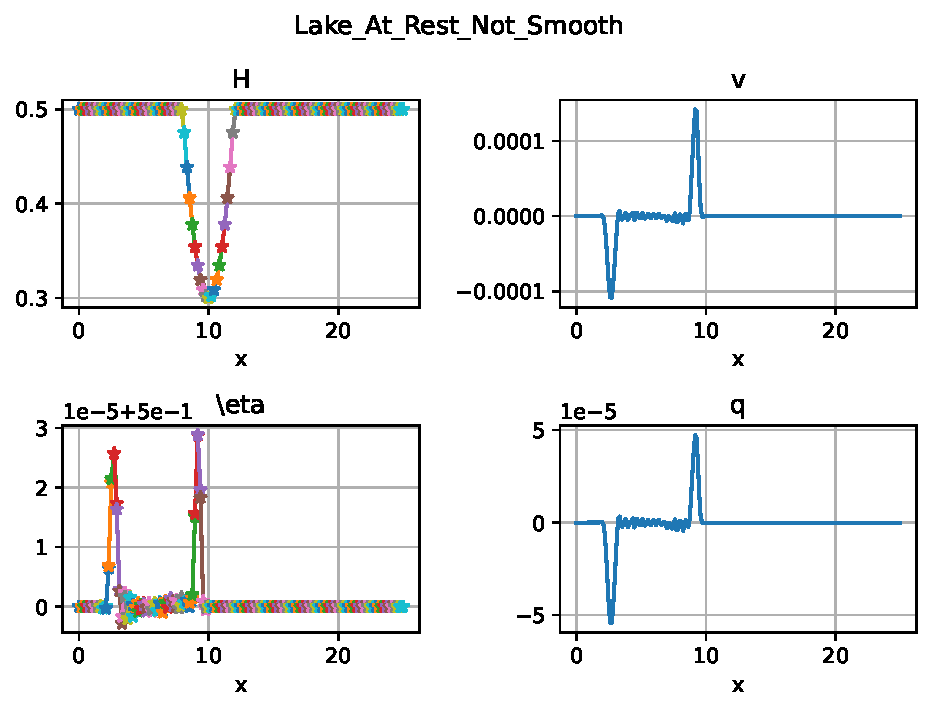
\includegraphics[trim= 0 0 0 180, clip,width=\textwidth]{figures/LatRnS_P1P2_N_el00120.pdf}\caption{P1P2 120 elements}
	\end{subfigure}\\
	\begin{subfigure}{0.60\textwidth}
		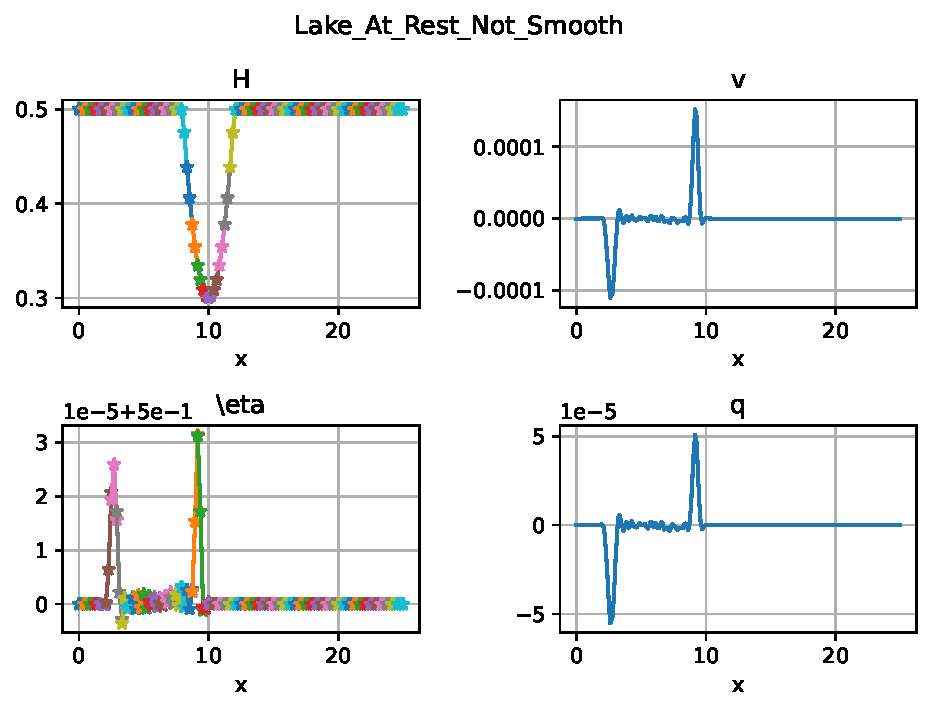
\includegraphics[trim= 0 0 0 180, clip,width=\textwidth]{figures/LatRnS_P2P3_N_el00060.pdf}\caption{P2P3 60 elements}
	\end{subfigure}\\
	\begin{subfigure}{0.60\textwidth}
		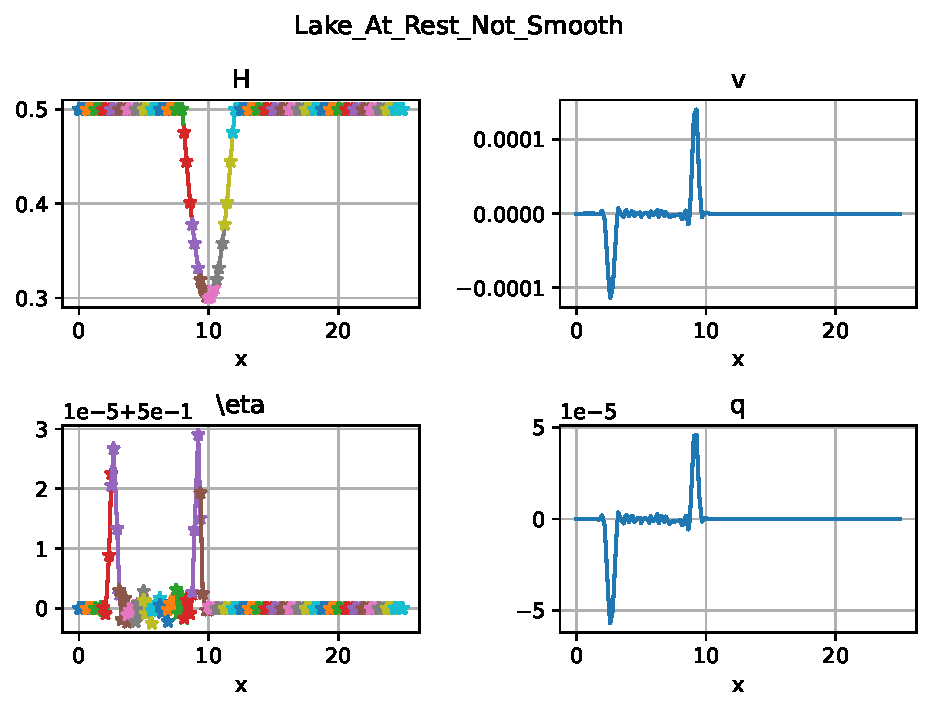
\includegraphics[trim= 0 0 0 180, clip,width=\textwidth]{figures/LatRnS_P3P4_N_el00040.pdf}\caption{P3P4 40 elements}
	\end{subfigure}\\
	\begin{subfigure}{0.60\textwidth}
		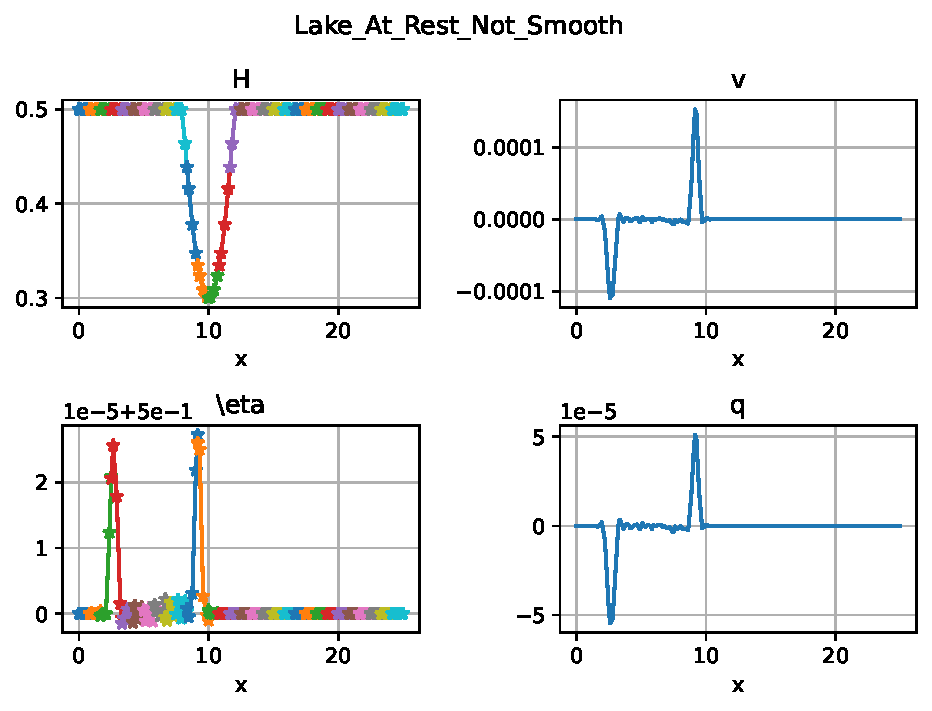
\includegraphics[trim= 0 0 0 180, clip,width=\textwidth]{figures/LatRnS_P4P5_N_el00030.pdf}\caption{P4P5 30 elements}
	\end{subfigure}
	\caption{Perturbation of lake at rest: initial condition and results}\label{fig:LatR_perturbation}
\end{figure}



\subsection{Shocks}
We are stuck here at the moment. I consider Sod in the domain $\Omega:=(0,1)$
\begin{align}
	H(x,0):=\begin{cases}
		1, \quad \text{if}~x\leq 0.5,\\
		0.2, \quad \text{otherwise},		
	\end{cases} \quad v(x,0)\equiv 0,
\end{align}
with Dirichlet boundary conditions. The final time is set to be $T_f:=0.1.$

The results are consistent but there is some oscillation in $v$ and I cannot get rid of it.





\bibliography{sn-bibliography}
\bibliographystyle{plain}



\end{document}
